\documentclass[12pt,german]{article}
\usepackage{listings}
%\usepackage[utf8]{inputenc}
\usepackage{inputenc}
\usepackage{graphicx}
\usepackage{float}

\lstset{
extendedchars=\true,
language=JAVA,
%inputencoding=utf8,
%basicstyle=\ttfamily,
%basicstyle=\ttfamily\fontsize{8}{8},
%commentstyle=\ttfamily\fontsize{8}{8},
basicstyle=\tiny;
columns=fullflexible,
%xleftmargin=5pt,
frame=single,
breaklines=true,
postbreak=\mbox{{$\hookrightarrow$}\space},
}
\renewcommand{\thesubsubsection}{\alph{subsubsection} )}
%\renewcommand{\thesubsubsection}{\thesubsection.\alph{subsubsection} )}

\begin{document}

\title{Übungsaufgaben I, SBV1 }
\author{Lisa Panholzer, Lukas Fiel}
\maketitle


\newpage
\section{Übungsaufgaben I}
\subsection{Gauss Filter}
\subsubsection{Implementierung}
\label{sec:Gausfilterimplementierung}
Es wurde ein Gauss Filter als ImageJ Filter implementiert. Die Behandlung der Randpixel wurde aus der Lehrveranstaltung übernommen. Gemeinsam mit dem Vortragenden Gerald Zwettler wurde die Java Klasse \textit{ConvolutionFilter} erweitert um auch die Randbereiche eines Bildes angemessen zu behandeln. In Heimarbeit wurde die Klasse um die Methode \textit{GetGaussMask} erweitert. In dieser wird die Verteilung einer Gauss Kurve auf eine 2 dimensionale Maske übertragen. \\

\lstinputlisting[frame=single,language=JAVA,breaklines=true]{../Gauss_.java}
\lstinputlisting[frame=single,language=JAVA,breaklines=true]{../ConvolutionFilter.java}



\subsubsection{Darstellung der Gauss-Maske mittels Surface-Plot}
Anschließend wurde eruiert welches Verhältnis von Sigma zum Radius der Maske eine klar zu erkennende Glocke darstellte. $ \frac{2}{4} $ hat die gewünschte Eigenschaft. 
\begin{table}[H]
  \centering
  \begin{tabular}{| c | c | c |}
    \hline
    $ \frac{sigma}{radius} $ & Masken Surface Plot & gefiltertes Bild \\
    \hline
    $ \frac{1}{4} $ &
	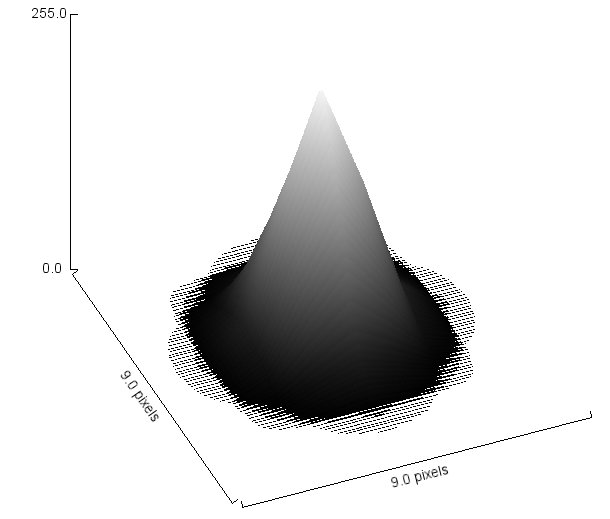
\includegraphics[width=4cm]{../testData/Gauss/GaussBellR4S1.jpg} & 	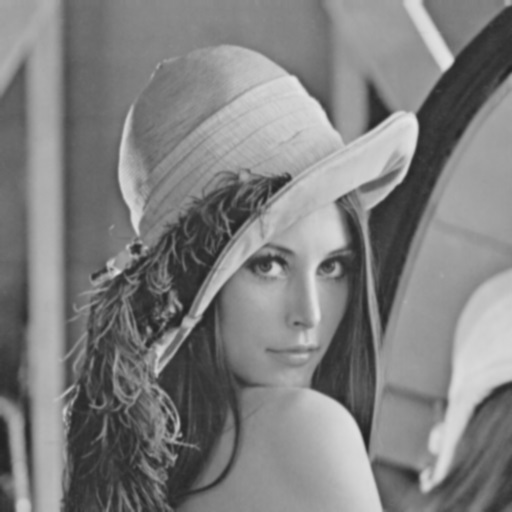
\includegraphics[width=4cm]{../testData/Gauss/LenaR4S1.jpg} \\
	    \hline
    $ \frac{2}{4} $ &
	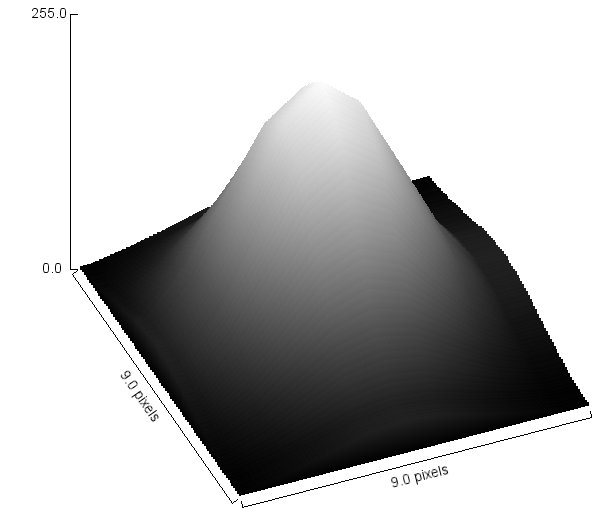
\includegraphics[width=4cm]{../testData/Gauss/GaussBellR4S2.jpg} & 	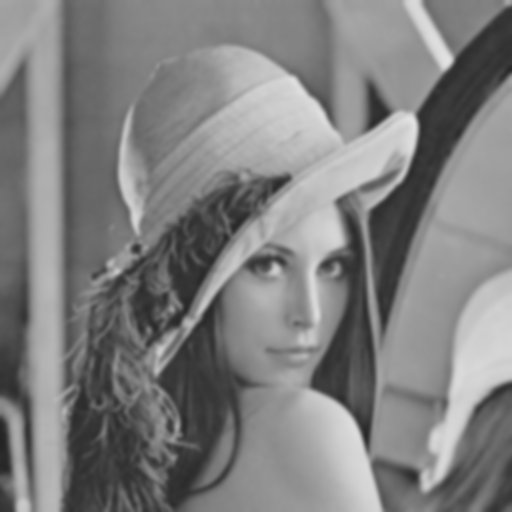
\includegraphics[width=4cm]{../testData/Gauss/LenaR4S2.jpg} \\
	    \hline
    $ \frac{3}{4} $ &
	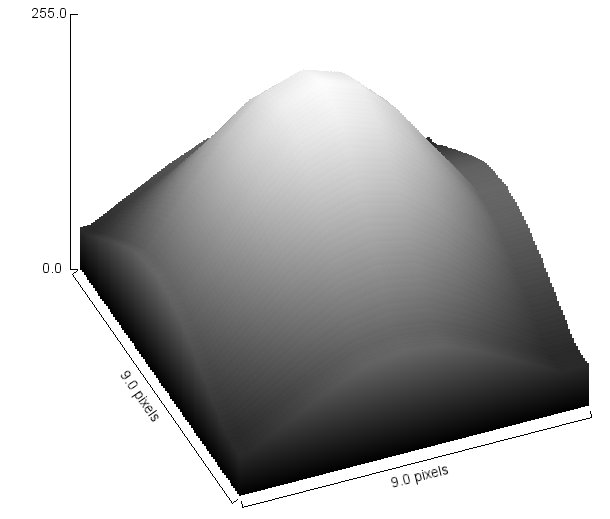
\includegraphics[width=4cm]{../testData/Gauss/GaussBellR4S3.jpg} & 	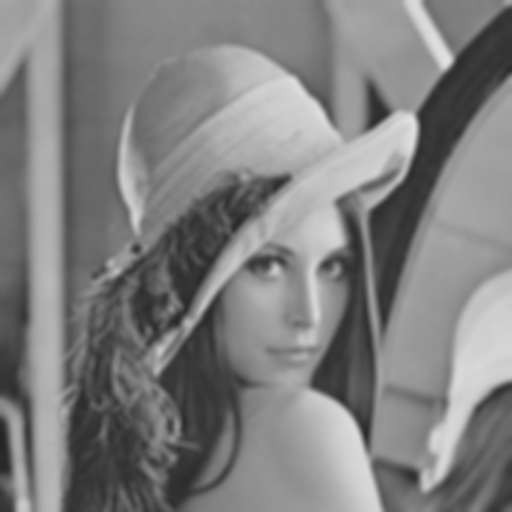
\includegraphics[width=4cm]{../testData/Gauss/LenaR4S3.jpg} \\
	    \hline
    $ \frac{4}{4} $ &
	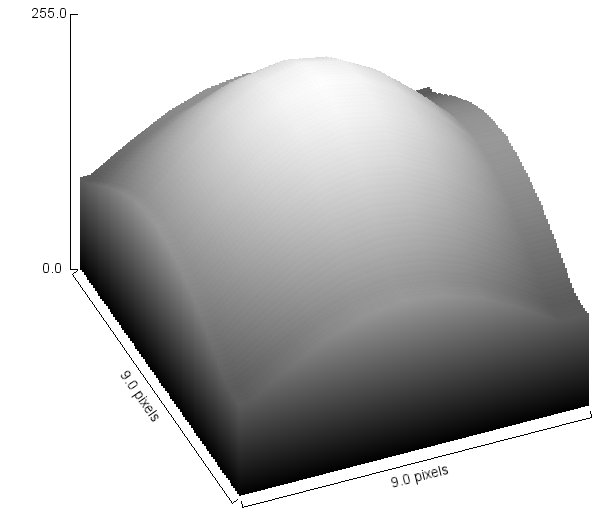
\includegraphics[width=4cm]{../testData/Gauss/GaussBellR4S4.jpg} & 	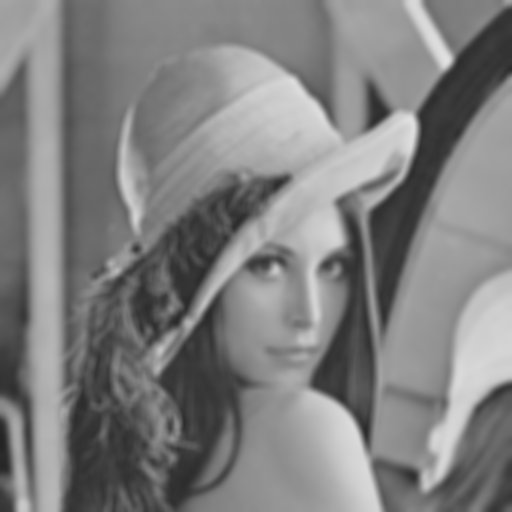
\includegraphics[width=4cm]{../testData/Gauss/LenaR4S4.jpg} \\
  \end{tabular}
  \caption{Gauss Filter Größen}
  \label{tab:GaussFilterGroessen}
\end{table}

\subsubsection{Auswirkungen im Bereich von Kanten und ansteigenden Intensitäten}
Weiters wurde der Übergang von scharfen Kanten und Verläufen mit dem Gauss Filter gefiltert. Man bemerkt gut, dass bei einem Intensitätsverlauf kaum ein Filtereffeckt sichtbar ist, während Kanten deutlich verschwommen erscheinen. Gewähltes Verhältnis: $ \frac{sigma}{radius} = \frac{2}{4} $
\begin{table}[H]
  \centering
  \begin{tabular}{| c | c | c |}
    \hline
    $ \frac{sigma}{radius} $ & Masken Surface Plot & gefiltertes Bild \\
    \hline
    $ \frac{1}{4} $ &
	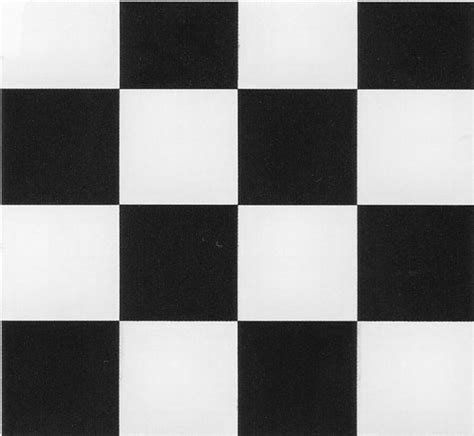
\includegraphics[width=4cm]{../testData/Gauss/Schachbrett.jpg} & 	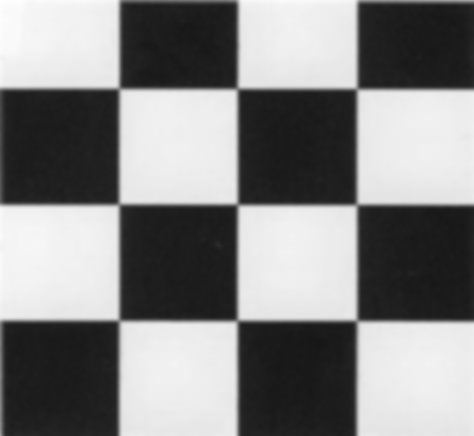
\includegraphics[width=4cm]{../testData/Gauss/SchachbrettR4S2.jpg} \\
	    \hline
    $ \frac{2}{4} $ &
	
\includegraphics[width=4cm]{../testData/Gauss/Regenbogen.jpg} & 	
\includegraphics[width=4cm]{../testData/Gauss/RegenbogenR4S2.jpg} \\
  \end{tabular}
  \caption{Gauss Filter Evaluierung}
  \label{tab:GaussFilterEvaluierung}
\end{table}
Interessant ist der Unterschied zum Median-Filter des nächsten Beispiels.Dieser stellt Kanten viel dutlicher dar und macht auch bei glatten Übergängen kaum einen bemerkenswerten Effeckt.



\begin{table}[H]
	\centering
	\begin{tabular}{|c  | c | c |}
    
    \hline
    $ \frac{sigma}{radius} $ & Gauss gefiltertes Bild & Median gefiltertes Bild \\
    \hline
    $ \frac{1}{4} $ &
	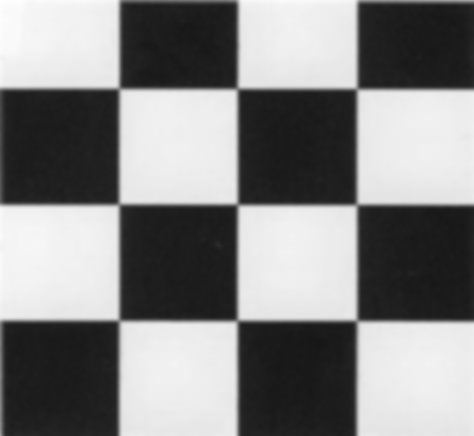
\includegraphics[width=4cm]{../testData/Gauss/SchachbrettR4S2.jpg} & 	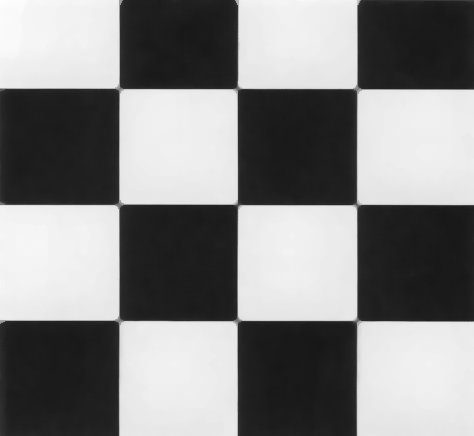
\includegraphics[width=4cm]{../testData/Median/SchachbrettR4.jpg} \\
	    \hline
    $ \frac{2}{4} $ &
	
\includegraphics[width=4cm]{../testData/Gauss/RegenbogenR4S2.jpg} & 	
\includegraphics[width=4cm]{../testData/Median/RegenbogenR4.jpg} \\
  \end{tabular}
  \caption{Gauss Filter vs. Median Filter}
  \label{tab:GaussMedianFilterEvaluierung}
\end{table}


%% -------------------------------------------------------------------------------------------------------------------------
%% ------------------------------------------- ZWEITES BEISPIEL -----------------------------------------------------
%% -------------------------------------------------------------------------------------------------------------------------
\newpage
\subsection{MedianFilter}
\subsubsection{Implementierung)}

Der MedianFilter kann leider nicht mittels der Klasse \textit{ConvolutionFilter} implementiert werden, da die Maske für dieses Vorgehen konstant sein müsste. Das Prinzip ist allerdings sehr ähnlich. Es wird ein Pixel in Mitten einer quadratischen Umgebung betrachtet. Dieses Pixel soll im resultierenden Bild als der Median Wert der Umgebung gesetzt werden. \\
Implementiert wurde dies durch das Herausschneiden der interessanten Umgebung aus einer Kopie des Ursprungsbildes und anschließender Medianwertberechnung. 

\lstinputlisting[frame=single,language=JAVA,breaklines=true]{../Median_.java}

\begin{table}[H]
  \centering
  \begin{tabular}{| c | c |}
    \hline
 	 Median gefiltertes Schachbrett & Median gefilterte Bild "Lena" \\
    \hline
	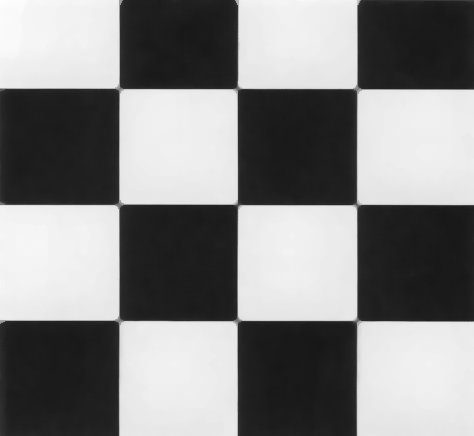
\includegraphics[width=4cm]{../testData/Median/SchachbrettR4.jpg} & 	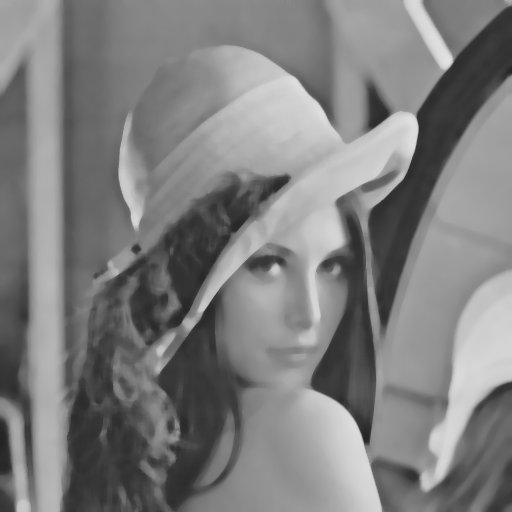
\includegraphics[width=4cm]{../testData/Median/LenaMedian.jpg} \\
	\hline
  \end{tabular}
  \caption{Median Filter}
  \label{tab:MedianFilter}
\end{table}

\subsubsection{4x4 Segment Darstellung und Statistische Werte}
\begin{figure}[H]
\centering
	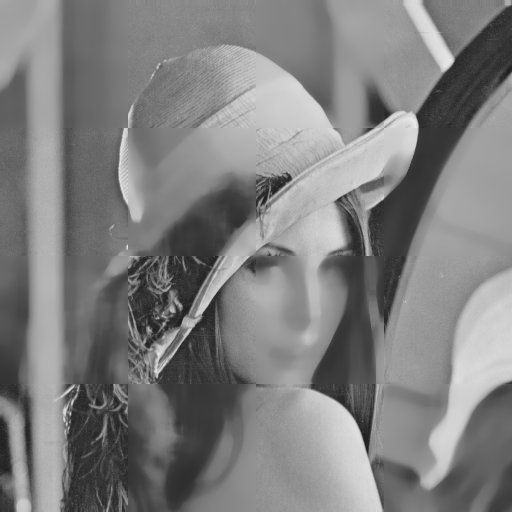
\includegraphics[width=10cm]{../testData/Median/4x4LenaR8.jpg}
	\caption{4x4 Darstellung des Originalbildes überlagert mit Segmenten des gefilterten Bildes}
    \label{tab:checkerboard}
\end{figure}
\begin{table}[H]
  \centering
  \begin{tabular}{| c | c |}
    \hline
 	 Originalbild & gefiltertes Bild $radius = 8$ \\
    \hline
	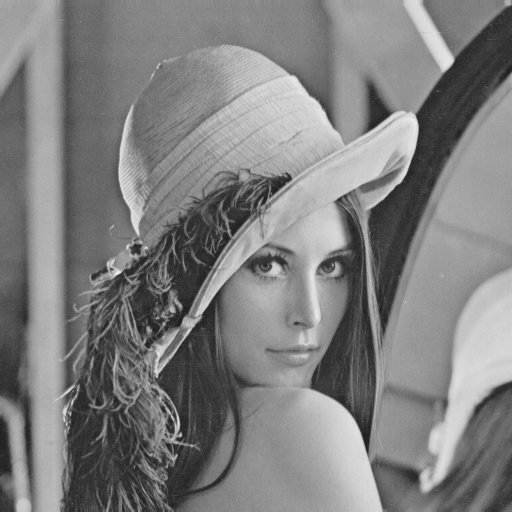
\includegraphics[width=4cm]{../testData/Lena.jpg} & 	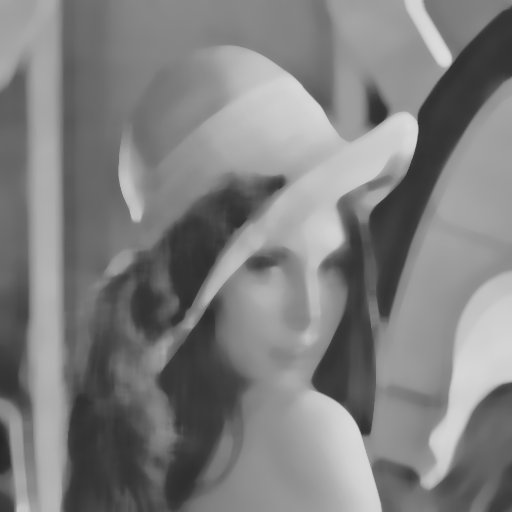
\includegraphics[width=4cm]{../testData/Median/LenaMedianR8.jpg} \\
	\hline
	Mean: 127.46 & Mean: 127.45 \\
	StdDev: 46.6 & StdDev: 44.1 \\
	Min: 29      & Min: 38      \\
	Max: 243     & Max: 220     \\
	\hline
  \end{tabular}
  \caption{Statistische Auswertung}
  \label{tab:Statistics}
\end{table}


\subsubsection{Salt \& Pepper Rauschen}
Der Salt \& Pepper Filter wird auf ein Testbild so oft angewendet, bis die Anzahl der Rausch-Pixel den Anteil der ursprünglichen Bild-Pixel übersteigt. Dies wird ca. bei einem Rausch-Anteil von über 50\% stattfinden. Da bei der Anwendung des Median-Filters immer der mittlerste Maskenwert herangezogen wird, kann bei einem Rausch-Anteil von über 50\% nur mehr Schwarz oder Weiß auftreten. Ab diesem Zeitpunkt kann der Median-Filter die Störsignale des Salt \& Pepper Filter nicht mehr korrigieren.


\begin{table}[H]
  \centering
  \begin{tabular}{| c | c | c |}
	\hline	
	ein bisschen verrauscht & sehr verrauscht &  fast unkenntlich  \\
    \hline
	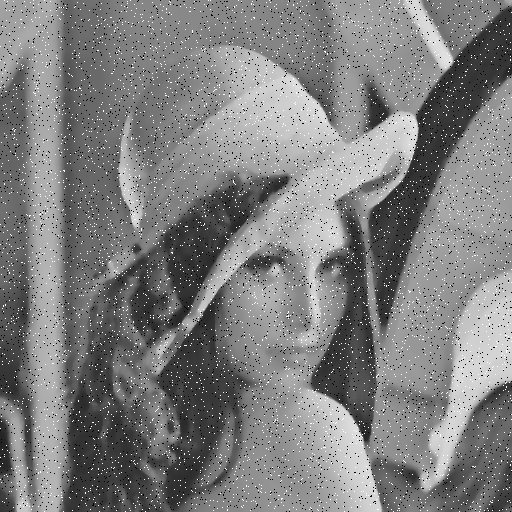
\includegraphics[width=4cm]{../testData/Median/LenaLittleNoise.jpg} & 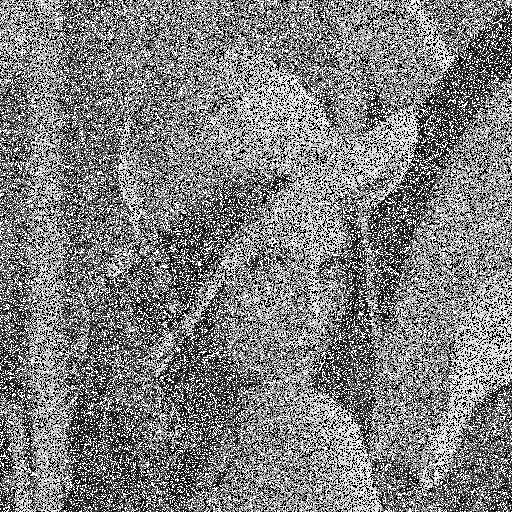
\includegraphics[width=4cm]{../testData/Median/LenaNoise.jpg} & 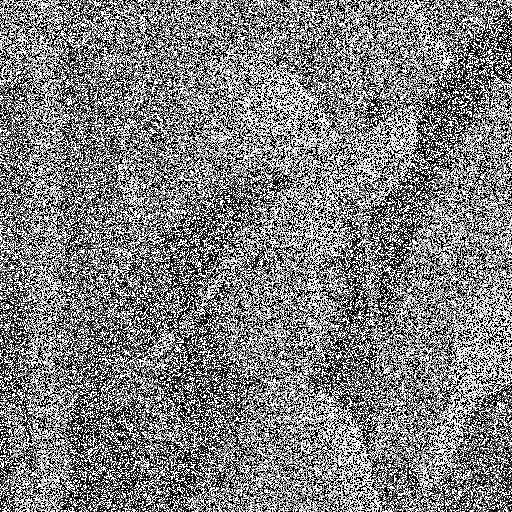
\includegraphics[width=4cm]{../testData/Median/LenaNoisyNoise.jpg} \\ 
	\hline
	normaler Filtereffeckt & erste Fehldarstellungen & ganze Bereiche sind schwarz/weiß \\
	\hline
	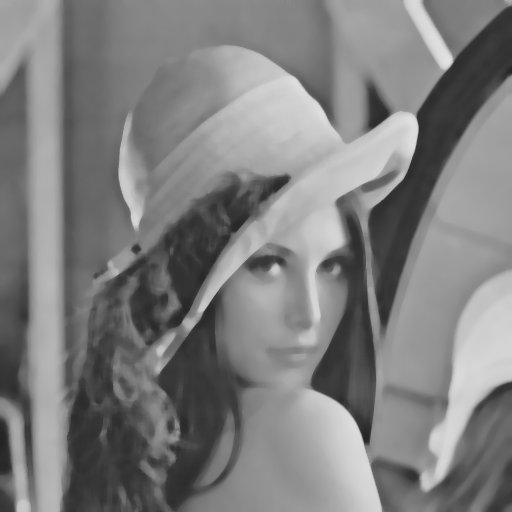
\includegraphics[width=4cm]{../testData/Median/LenaMedian.jpg} & 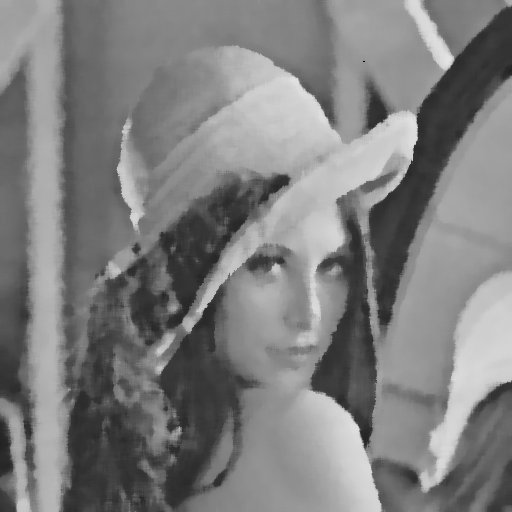
\includegraphics[width=4cm]{../testData/Median/LenaNoiseR4.jpg} & 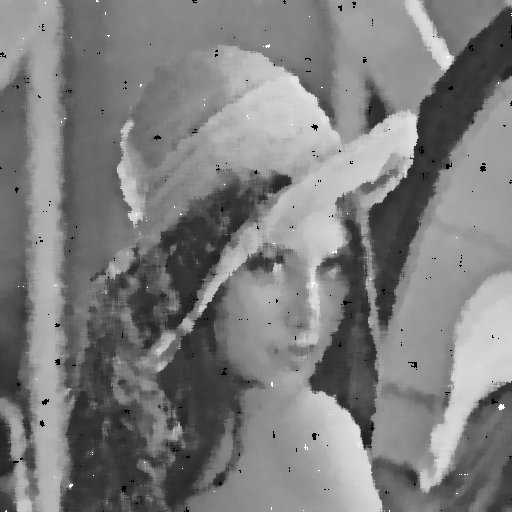
\includegraphics[width=4cm]{../testData/Median/LenaNoisyNoiseR4.jpg} \\
	\hline

  \end{tabular}
  \caption{Amwendung des Median Filters auf Bilder die mit Salt Pepper Noise verschlechtert wurden.}
  \label{tab:Statistics}
\end{table}





%% -------------------------------------------------------------------------------------------------------------------------
%% ------------------------------------------- DRITTES BEISPIEL -----------------------------------------------------
%% -------------------------------------------------------------------------------------------------------------------------
\newpage
\subsection{Steuerung des Filtereffekts }

\subsubsection{Vergleich}
Das selbstgeschriebene Plugin \textit{FiltereffektEvaluierung\_} wurde geschrieben um die Laufzeiten der einzelnen Filter zu erfassen. Hierbei wurde darauf geachtet, dass mittels der Methode \textit{System.nanoTime()} im Gegensatz zu \textit{System.millis()} einge genauere Zeitmessung möglich ist. Als eine sehr große Maske wurde $  radius = 40 $ gewählt. Das Setzen der Größe $ sigma $ ist bei der Messung der Laufzeit irrelevant, da sie nur für das initiale Erstellen der Maske ausschlaggebend ist. \\

Ein Vergrößern der Maske steigert die benötigte Rechenzeit enorm. Man erkennt auch gut, dass eine große Filtermaske nicht unbedingt mit einem enormen Filtereffekt zu tun haben muss. Da hier ein kleines $sigma$ gewählt wurde, ist auch die Auswirkung des Filters nicht groß, aber deutlich von der des Filters mit der kleinen Maske unterscheidbar.


Zusätzlich zur Klasse \textit{FiltereffektEvaluierung\_.java} werden auch viele der anderen in diesem Papier besprochenen Klassen benötigt.
\lstinputlisting[frame=single,language=JAVA,breaklines=true]{../FiltereffektEvaluierung_.java}

Die so gewonnenen Daten wurden in eine Excel Tabelle eingetragen und in Diagrammen dargestellt. 
\begin{figure} [H]
  \centering
  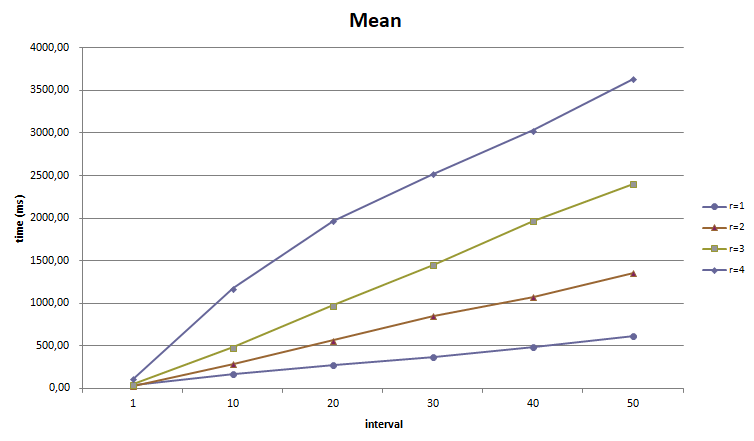
\includegraphics[width=12cm]{TimeEvaluationGraph_Mean.png}
  \caption{Der Mean Filter wirde mit verschiedenen Radien wiederholt Ausgeführt und dabei die Laufzeit gemessen.}
  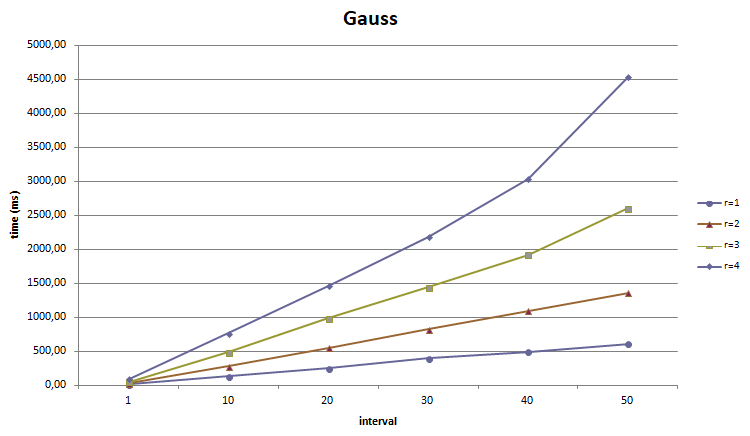
\includegraphics[width=12cm]{TimeEvaluationGraph_Gauss.png}
  \caption{Der Gauss Filter wirde mit verschiedenen Radien wiederholt Ausgeführt und dabei die Laufzeit gemessen.}
\end{figure}



3D Masken könnten neben dem Filtereffekt zum Beispiel bei einem RGB Bild auch Farbtöne verstärken/abschwächen. Dabei müsen aber im Falle des Median-Filters für jeden Pixel des dreidimensionalen Bildes alle 3 Dimensionen der Maske berechnet werden. Bei Mean- und Gauss-Filter hingegen reicht es einen zweidimensionalen Filter auf jede Ebene der dritten Dimension anzuwenden und die Ergebisse weiterzuverarbeiten. 


\begin{center}
	$t_{gP} ... time to get pixel value. Die Zeit einen Pixel aus der Berechnung mit einer 2D Maske  $ \\
	$t_{cM} ... time to caluclate initial Mask$ \\
	$t_{cMM} ... time to calculate MedianMask $ \\
	$d ... Anzahl der Dimensionen$ \\
\end{center}

\subsubsection{Diskussion der Ergebnisse}
Mehrmaliges Anwenden eines Filters ma
\begin{figure} [H]
  \centering
  \begin{tabular}{| c | c | c | c |}
    \hline
    ein mal gefiltert & zwei mal gefiltert & drei mal gefiltert & vier mal gefiltert \\
    \hline
	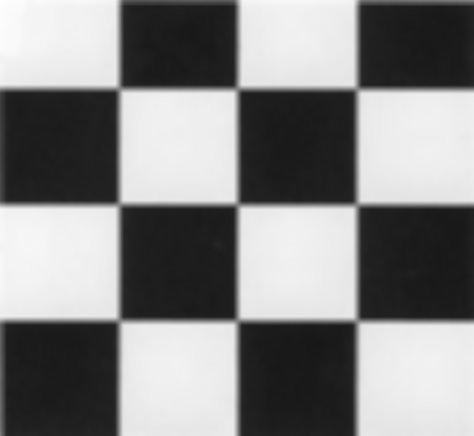
\includegraphics[width=3cm]{../testData/Gauss/SchachbrettR4S4v1.jpg} & 	
	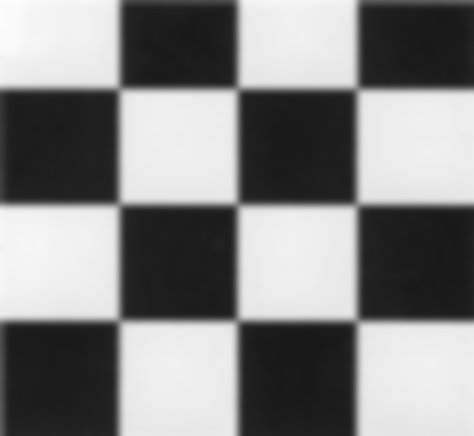
\includegraphics[width=3cm]{../testData/Gauss/SchachbrettR4S4v2.jpg} &
	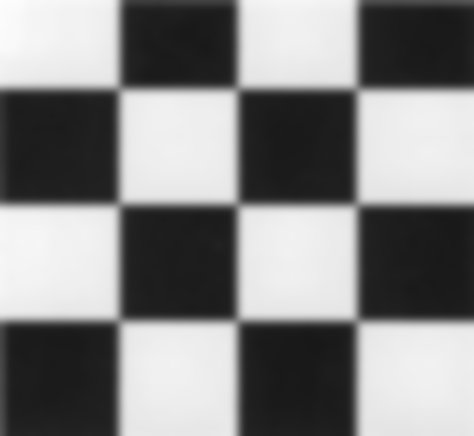
\includegraphics[width=3cm]{../testData/Gauss/SchachbrettR4S4v3.jpg} & 	
	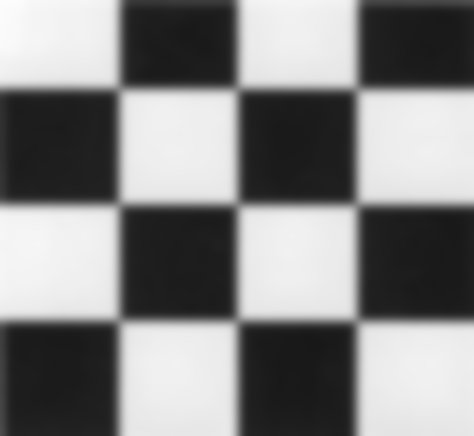
\includegraphics[width=3cm]{../testData/Gauss/SchachbrettR4S4v4.jpg} \\
	    \hline
	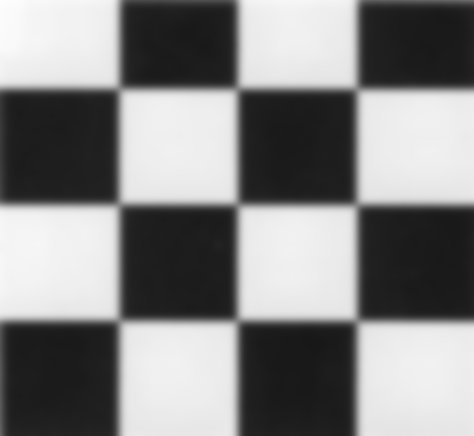
\includegraphics[width=3cm]{../testData/Gauss/SchachbrettR40S4v1.jpg} & 	
	
\includegraphics[width=3cm]{../testData/Gauss/SchachbrettR40S4v2.jpg} &
	
\includegraphics[width=3cm]{../testData/Gauss/SchachbrettR40S4v3.jpg} & 	
	
\includegraphics[width=3cm]{../testData/Gauss/SchachbrettR40S4v4.jpg} \\
	\hline
  \end{tabular}
  \caption{Wiederholte Anwendung des Gauss Filters mit $ radius = 4 $ (oben) und $radius = 40 $ (unten)}
  \label{tab:wiederholterGauss}


\end{figure}

%% -------------------------------------------------------------------------------------------------------------------------
%% ------------------------------------------- VIERTES BEISPIEL -----------------------------------------------------
%% -------------------------------------------------------------------------------------------------------------------------
\newpage
\section{Histogrammeinebnung  }

\subsubsection{a) Ablauf und Lösungsidee}
 Die Histogrammeinebnung wurde mit der, wie im Foliensatz beschriebenen, Formel durchgeführt. Die genaue Implementierung findet sich im Bereich "Code". 
\subsubsection{a) Tests}
Die Implementierung wurde anhand der folgenden drei Bilder getestet:
\begin{enumerate}
\item Strand: 
Das Bild "Strand" (siehe Figure \ref{fig:Strand01}) enthält eine halbwegs gleichmäßige Verteilung der Grautöne. Nach Anwendung der Histogrammeinebnung  (siehe Figure \ref{fig:Strand02}) kann man eine Verstärkung des Kontrastes erkennen.
\begin{figure}[H] \centering
	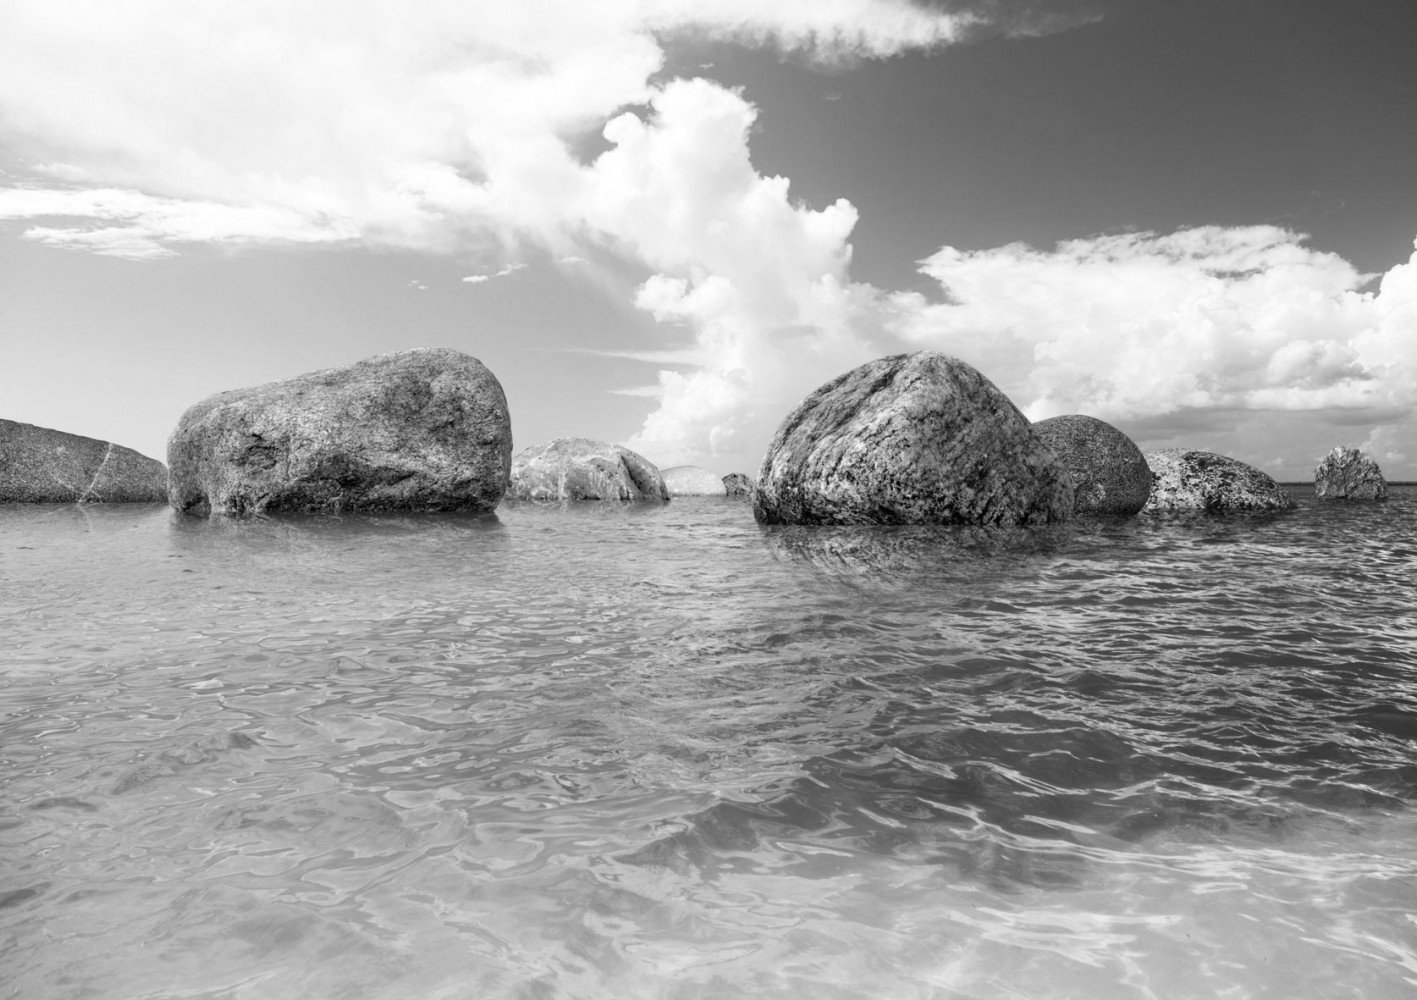
\includegraphics[width=7cm]{../testData/Results/Strand/Strand.jpg}
	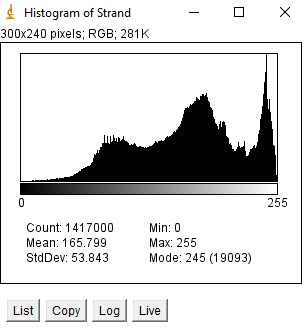
\includegraphics[width=4cm]{../testData/Results/Strand/Strand-histogram.png}
	\caption{Original Test-Bild "Strand" mit dazugehörigem Histogramm}
	 \label{fig:Strand01}
\end{figure}
\begin{figure}[H] \centering
	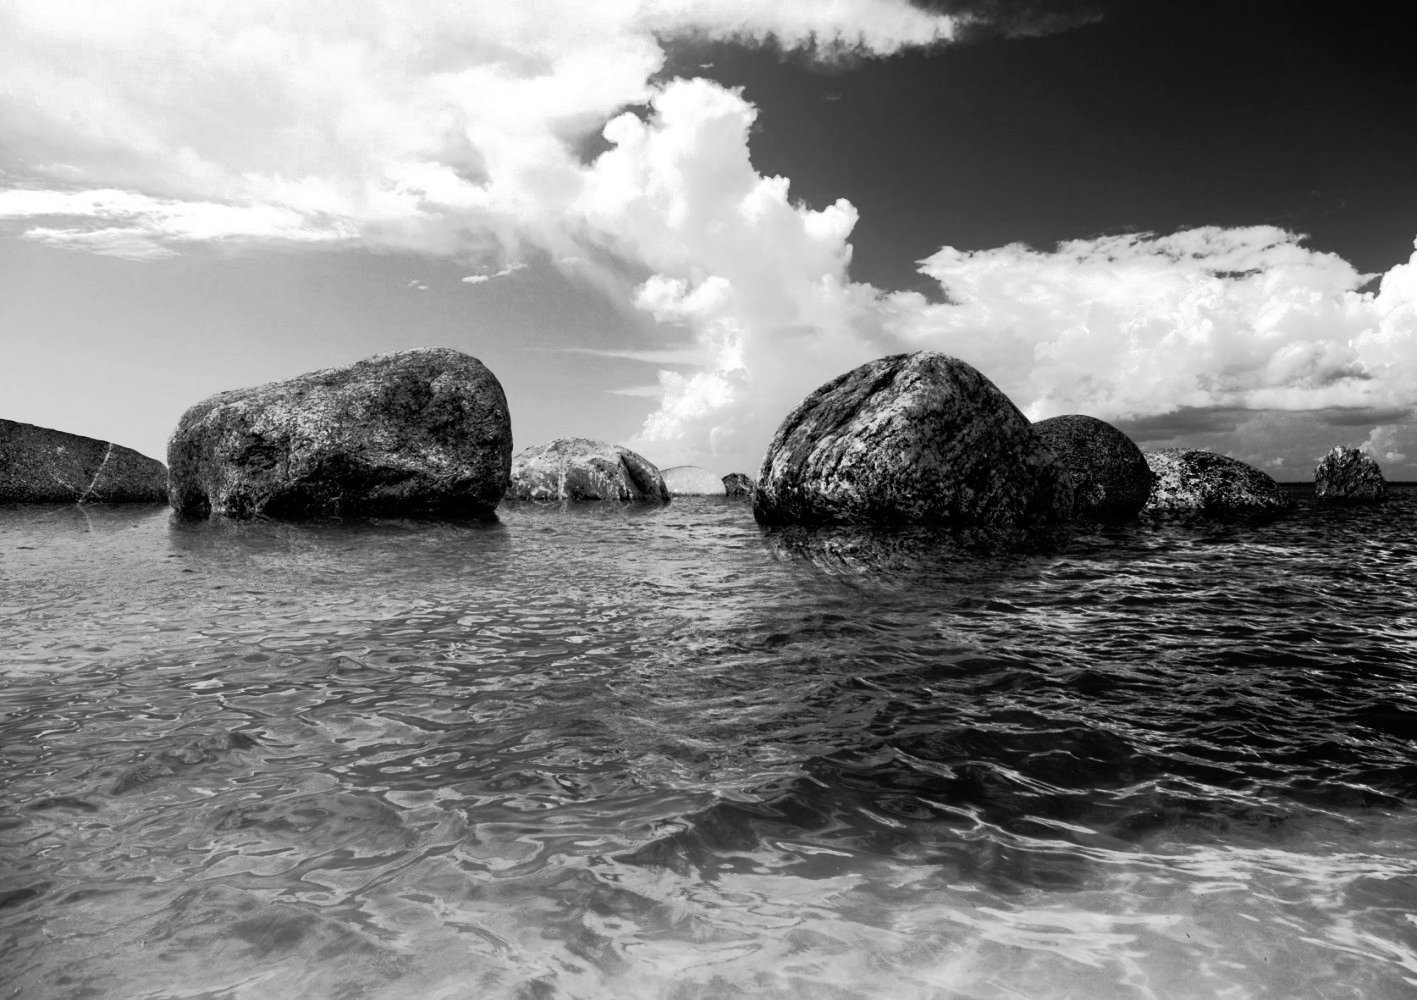
\includegraphics[width=7cm]{../testData/Results/Strand/Strand-equalized.jpg}
	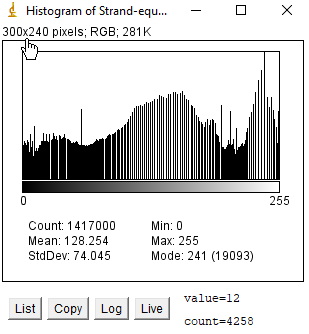
\includegraphics[width=4cm]{../testData/Results/Strand/Strand-equalized-histogram.png}
	\caption{Test-Bild "Strand" mit dazugehörigem Histogramm nach der Histogrammeinebnung}
	 \label{fig:Strand02}
\end{figure}

\item Russland: 
Das Bild "Russland"  (siehe Figure \ref{fig:Russland01}) enthält sehr wenig Kontrast und viele der Grautöne sind im Histogram benachbart. Nach der Anwendung der Histogrammeinebnung  (siehe Figure \ref{fig:Russland02}) verstärkt sich der Kontrast um ein vielfaches und selbst die Wokenformation sind nun detailliert sichtbar.
\begin{figure}[H] \centering
	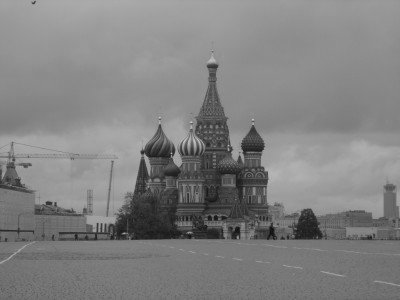
\includegraphics[width=7cm]{../testData/Results/Russland/Russland.jpg}
	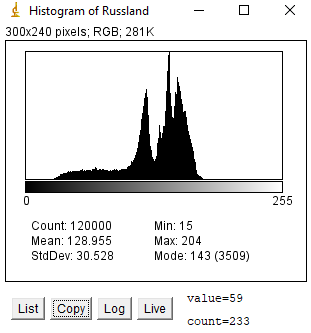
\includegraphics[width=4cm]{../testData/Results/Russland/Russland-histogram.png}
	\caption{Original Test-Bild "Russland" mit dazugehörigem Histogramm}
	 \label{fig:Russland01}
\end{figure}
\begin{figure}[H] \centering
	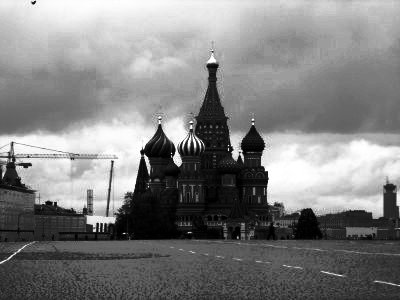
\includegraphics[width=7cm]{../testData/Results/Russland/Russland-equalized.jpg}
	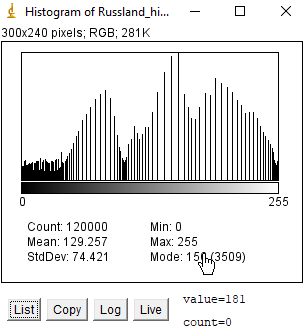
\includegraphics[width=4cm]{../testData/Results/Russland/Russland-equalized-histogram.png}
	\caption{Test-Bild "Russland" mit dazugehörigem Histogramm nach der Histogrammeinebnung}
	 \label{fig:Russland02}
\end{figure}

\item Landschaft: 
Das Bild "Landschaft"  (siehe Figure \ref{fig:Landschaft01}) hat im Vergleich zu den ersten beiden Testbildern einen höheren Kontrast und ist dunkler. Bei der Anwendung der Histogrammeinebnung  (siehe Figure \ref{fig:Landschaft02}) kann man nun beobachten, das aufgrund der Gleichverteilung der Grautöne Richtung den Maximalwert (255), das Bild sich aufhellt und der Kontrast erhalten bleibt.
\begin{figure}[H] \centering
	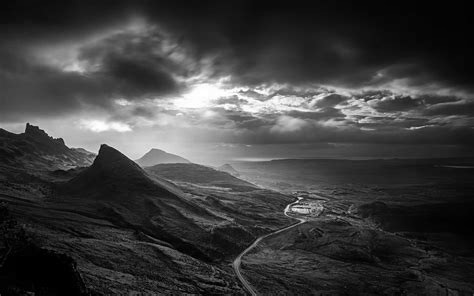
\includegraphics[width=7cm]{../testData/Results/Landschaft/Landschaft.jpg}
	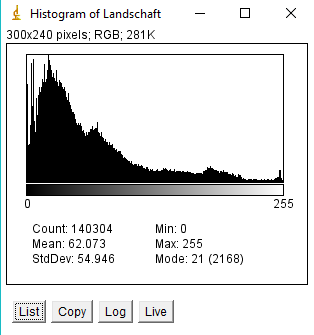
\includegraphics[width=4cm]{../testData/Results/Landschaft/Landschaft-histogram.png}
	\caption{Original Test-Bild "Landschaft" mit dazugehörigem Histogramm}
	 \label{fig:Landschaft01}
\end{figure}
\begin{figure}[H] \centering
	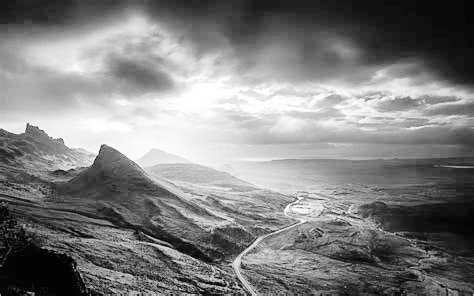
\includegraphics[width=7cm]{../testData/Results/Landschaft/Landschaft-equalized.jpg}
	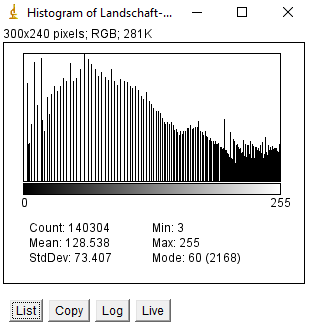
\includegraphics[width=4cm]{../testData/Results/Landschaft/Landschaft-equalized-histogram.png}
	\caption{Test-Bild "Landschaft" mit dazugehörigem Histogramm nach der Histogrammeinebnung}
	 \label{fig:Landschaft02}
\end{figure}


\end{enumerate}


\pagebreak
\subsection {b) Diskussion Histogrammeinebnung}
Es kann zu einer Verschlechterung der Bildqualität kommen, wenn die Histogrammeinebnung zum Beispiel auf ein stark überbelichtetes Bild angewandt wird. Bei dem Testbild "Straße mit Fußgängern"  (siehe Figure \ref{fig:Ueberbelichtung01}) sieht man, dass der Großteil der Pixelintensitäten ca. über 200 liegt. Findet nun die Einebnung  (siehe Figure \ref{fig:Ueberbelichtung02}) statt werden die Verläufe nicht mehr weich dargestellt. Die Unterschiede zwischen den Pixelintensitäten werden zu hoch und Teile des Bildes deshalb kantiger dargestellt.
\begin{figure}[H] \centering
	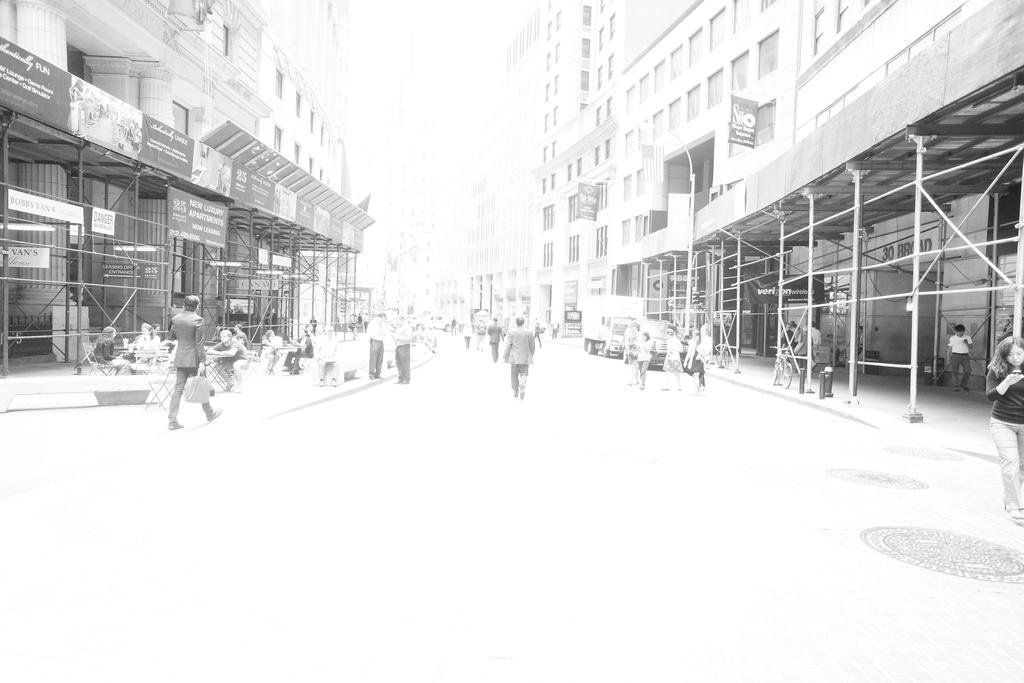
\includegraphics[width=7cm]{../testData/Results/Ueberbelichtung/Ueberbelichtung.jpg}
	\includegraphics[width=4cm]{../testData/Results/Ueberbelichtung/Ueberbelichtung-histogram.png}
	\caption{Original Test-Bild "Überbelichtung" mit dazugehörigem Histogramm}
	\label{fig:Ueberbelichtung01}
\end{figure}
\begin{figure}[H] \centering
	\includegraphics[width=7cm]{../testData/Results/Ueberbelichtung/Ueberbelichtung-equalized.jpg}
	\includegraphics[width=4cm]{../testData/Results/Ueberbelichtung/Ueberbelichtung-equalized-histogram.png}
	\caption{Test-Bild "Überbelichtung" mit dazugehörigem Histogramm nach der Histogrammeinebnung}
	\label{fig:Ueberbelichtung02}
\end{figure}
\pagebreak
\subsection{Code}
\lstinputlisting[frame=single,language=JAVA,breaklines=true]{../HistogramEqualization_.java}



%% -------------------------------------------------------------------------------------------------------------------------
%% ------------------------------------------- FÜNFTES BEISPIEL -----------------------------------------------------
%% -------------------------------------------------------------------------------------------------------------------------
\newpage
\section{ Raster-Entfernung im Frequenzraum}
\subsection{Workflow}
\begin{itemize}
	\item Starten von \textit{imageJ.exe}
	\item Öffnen eines Bildes
	\item \textit{Process $\rightarrow$ FFT $\rightarrow$ FFT}
	\item Zuschneiden des interessanten Bereichs im FFT Bild
	\item \textit{Process $\rightarrow$ FFT $\rightarrow$ inverse FFT}
\end{itemize}

\subsection{a) Beispiele}

\subsubsection{Auge}
Es wurde ein Bild gewählt, welches (wie bei einem Plakatdruck) Punkte in regelmässigen Abständen aufweist. Die eigentliche Bildinformation steckt in der Dicke der Punkte. Eine FFT zeigt deutlich ein periodisches Muster. Will man nun die eigentliche Bildinformation gewinnen, müssen hochfrequente Anteile des Bildes entfernt werden. Tabelle \ref{tab:AuswertungAuge} zeigt deutlich dass durch ein Entfernen der Randbereiche (höhere Frequenzen) im FFT Bild und die anschließende Rücktransformation die eigentliche Bildinformation gewonnen werden konnte.
\begin{table}[H]
  \centering
  \begin{tabular}{c | c}
    \hline
    Bild & FFT \\
    \hline
	\includegraphics[width=4cm]{../testData/Auge.jpg} & \includegraphics[width=4cm]{../testData/Results/Auge/FFT_of_Auge.jpg} \\
    \hline
    \includegraphics[width=4cm]{../testData/Results/Auge/reduced_Auge.jpg} & \includegraphics[width=4cm]{../testData/Results/Auge/reduced_FFT_of_Auge.jpg} \\
  \end{tabular}
  \caption{Auswertung Auge}
  \label{tab:AuswertungAuge}
\end{table}



\subsubsection{Elefant}
In diesem Bild sind viele periodisch auftretende Elemente enthalten. Es wurde versucht die Schrift, die Gitterstäbe im Hintergrund und natürlich die beiden Tiere gut sichtbar zu erhalten (siehe Tabelle \ref{tab:AuswertungElefant}). Da aber die Gitterstäbe selbst periodisch im Bild vorkommen und auch die Schrift sich wiederholende senkrechte Kanten hat, ist dies nicht einfach. Ein Auslöschen der horizontalen und vertikalen Anteile aus dem Bild brachte in unseren Versuchen das beste Ergebnis. Hierbei ist aber zu beachten, dass das Zentrum des FFT Bildes die meiste Information enthält. Daher wurde diese belassen. Auch die Randbereiche der FFT wurden belassen, da diese für scharfe Kanten im Bild verantwortlich sind. Ein Wegschneiden dieser Bereiche würde auch die Konturen des Elefanten und die Schrift unscharf machen.
\begin{table}[H]
  \centering
  \begin{tabular}{c | c}
    \hline
    Bild & FFT \\
    \hline
	\includegraphics[width=4cm]{../testData/Elefant.jpg} & \includegraphics[width=4cm]{../testData/Results/Elefant/FFT_of_Elefant.jpg} \\
    \hline
    \includegraphics[width=4cm]{../testData/Results/Elefant/reducedElefant.jpg} & \includegraphics[width=4cm]{../testData/Results/Elefant/reducedFFT_of_Elefant.jpg} \\
  \end{tabular}
  \caption{Auswertung Elefant}
  \label{tab:AuswertungElefant }
\end{table}

\subsubsection{Lochgitter}
Hier handelt es sich um ein perspektivisch beleuchtetes Lochgitter (siehe Tabelle \ref{tab:AuswertungLochgitter}). Die Löcher sind sechseckig. In der FFT erkennt man gut die Periodizität. Ein Wegschneiden der äusseren Bereiche der FFT und eine Rücktransformation zeigt deutlich die perspektivische Beleuchtung. Das Lochgitter konnte vollkommen entfernt werden. Es ist auch anzumerken, dass im rücktransformierten Bild eine Schrift \textit{"colourbox"} deutlich zu erkennen ist. Bei genauerer Betrachtung des Ursprungsbildes ist diese hinter dem Gitter zu erkennen.  
\begin{table}[H]
  \centering
  \begin{tabular}{c | c}
    \hline
    Bild & FFT \\
    \hline
	\includegraphics[width=4cm]{../testData/Lochgitter.jpg} & \includegraphics[width=4cm]{../testData/Results/Lochgitter/FFT_of_Lochgitter.jpg} \\
    \hline
    \includegraphics[width=4cm]{../testData/Results/Lochgitter/reducedLochgitter.jpg} & \includegraphics[width=4cm]{../testData/Results/Lochgitter/reducedFFT_of_Lochgitter.jpg} \\
  \end{tabular}
  \caption{Auswertung Lochgitter}
  \label{tab:AuswertungLochgitter}
\end{table}

\subsection{b) Analyse eines Frequenzmusters}
Ein sich wiederholendes Muster in einem Bild ist mittels \textit{FFT} gut vom eigentlichen Bildinhalt zu unterscheiden. So kann das Muster entfernt werden und das eigentliche Bild mittels \textit{inverseFFT} ermittelt werden.

Leider sind reale Bilder meist nicht genau horizontal ausgerichtet. Auch kann man nicht davon ausgehen, dass  wiederholende Elemente in der Realität unverzerrt in einem Bild dargestellt sind. Kanten werden nur in den seltensten Fällen genau durch einen Pixel des Bildes dargestellt. All diese Umstände machen es schwer aus einem Alltagsfoto wiederkehrende Elemente herauszufiltern. 

Um den Raster  möglichst gut zu entfernen sollten die Linien regelmäßig, in gleichen Abständen auf dem Bild vorhanden sein. Diese sollten auch sehr klar dargestellt werden, dann können diese möglichst exakt vom restlichen Bildinhalt getrennt werden.


\section{Anhang}
\lstinputlisting[frame=single,language=JAVA,breaklines=true]{../ConvolutionFilter.java}


\end{document}
